%\documentclass{acm_proc_article-sp}
\documentclass{article}
\usepackage{graphicx}

\pagestyle{empty}

\begin{document}

\clearpage
\begin{figure}[t!]
    \centering
    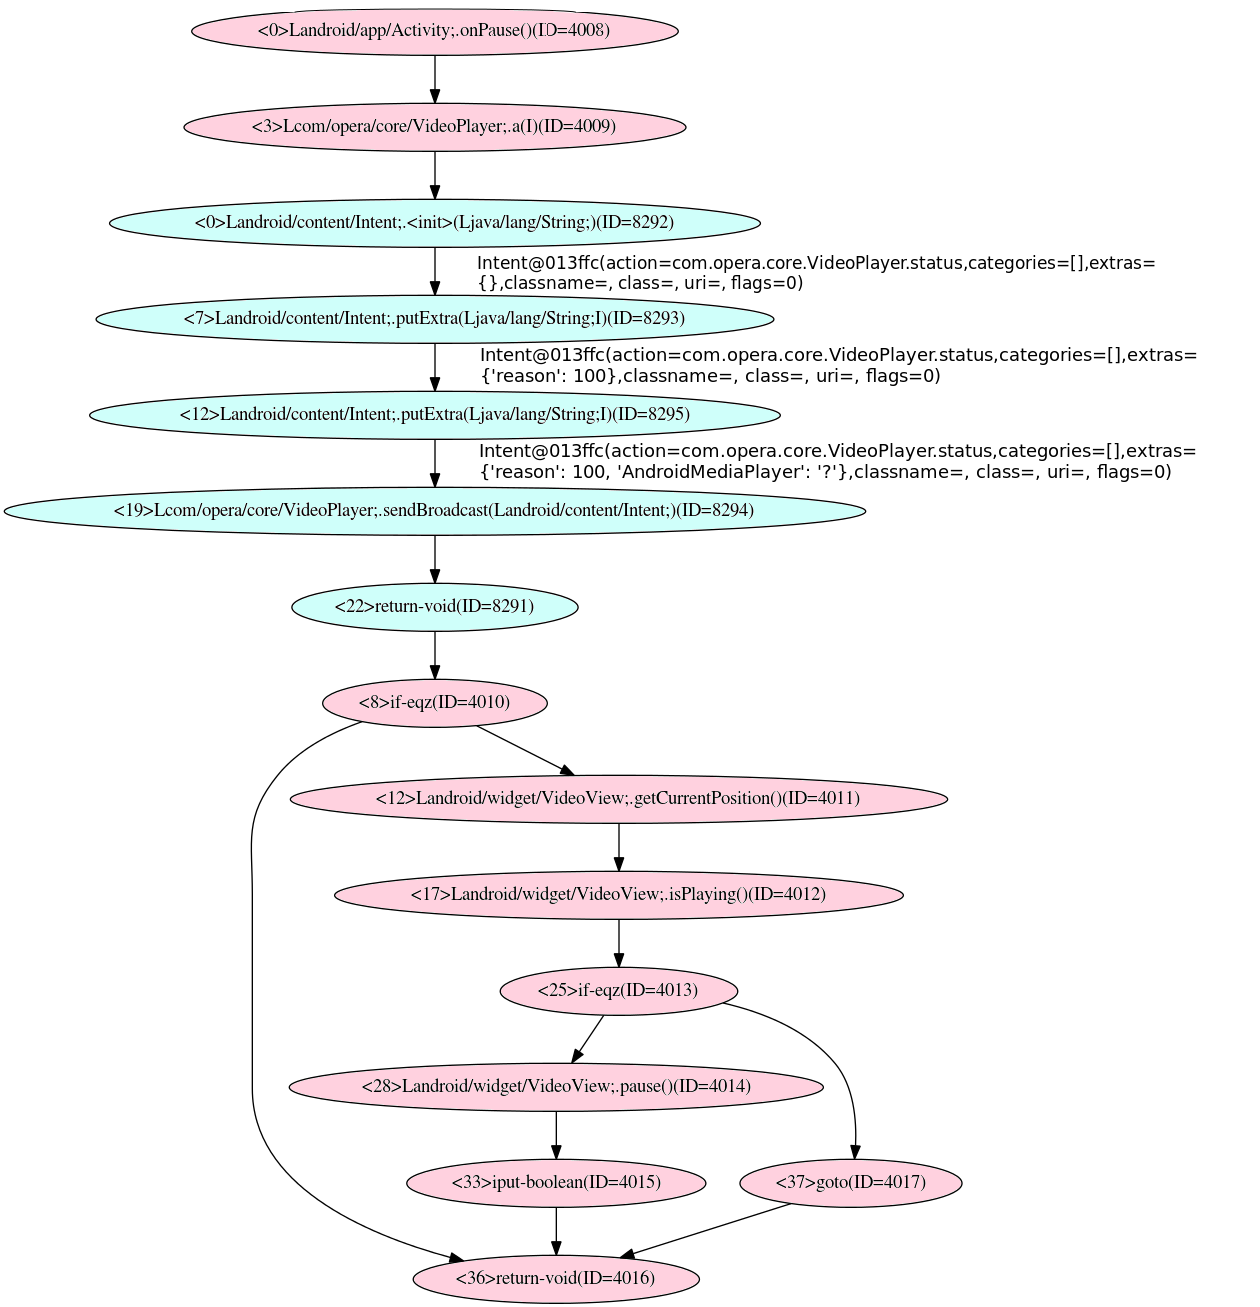
\includegraphics[scale=0.38]{figures/annotated}
    \caption{This diagram shows an example control flow graph. Each node
        represents a basic block, and is labeled by the last instruction within
        that basic block. Different colored nodes represent basic blocks from
        separate methods. For example, before expansion, basic block 4009 is
        connected to basic block 4010. After expansion, we splice in the nodes
    and edges from the invoked method's graph.}
    \label{example_analysis}
    \vspace*{6in}
\end{figure}

\begin{figure}[!htpb]
    \centering
    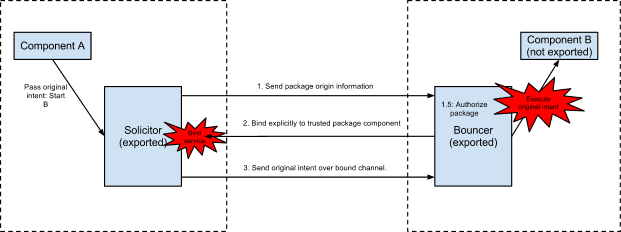
\includegraphics[scale=0.7]{figures/image00}
    \caption{Good Intention Library}
\end{figure}

\end{document}
